% pour genree un pdf: faire
% pdflatex exemple.tex
\documentclass{article}

%% Paquets LateX utiles

\usepackage[utf8]{inputenc} 		% encodage des caracteres utilise (pour les caracteres accentues) -- non utilise ici.
%\usepackage[latin1]{inputenc} 		% autre encodage
\usepackage[french]{babel}		% pour une mise en forme "francaise"
\usepackage{amsmath,amssymb,amsthm}	% pour les maths
\usepackage{graphicx}			% pour inclure des graphiques

\usepackage[hidelinks]{hyperref}
\usepackage{color}			% pour ajouter des couleurs dans vos textes
\usepackage{geometry}
\geometry{hmargin=2.5cm,vmargin=3cm}
\renewcommand{\contentsname}{\centering Contents}


\begin{document}
\begin{titlepage}
    \begin{flushleft}
    
\includegraphics[width=11em]{logo.png}\\[1.5cm]
    \end{flushleft}
    %\begin{sffamily}
    \begin{center}
        \textsc{{\LARGE \ Master Données, Apprentissage et Connaissances-DAC}}\\[4cm]
        \textsc{\Huge{RAPPORT PROJET MOGPL}}\\[1cm]
        \textsc{\Huge{DICE BATTLE}}\\[5.5cm]
        %\hspace{30pt}
            % Author and supervisor
        \begin{minipage}{1\textwidth}
            \begin{flushleft} \large
            \textsc{\LARGE{Realisé par :}}\\[0.5cm]
            \textsc{Djeddal Hanane}\\
            \textsc{Touzari Liticia}\\
            GROUPE 2\\
            \end{flushleft}
        \end{minipage}
        \vfill
    \end{center}
    %\end{sffamily}
  \end{titlepage}
  
\maketitle
\tableofcontents					% si on veut une table des matieres


\newpage


\section{Introduction}
\paragraph{}
    \begin{Large}
        La theorie des jeux est le domaine de mathématique qui permet la modélisation des interactions stratégiques. 
        Dans ce contexte, où plusieurs agents, dit joueurs, cherchent à maximiser leurs gains, le but est de trouver
        une stratégie optimale pour chaque joueur et d'envisager les eventuelles relations liant l'interêt de chauqe 
        joueur, et les possibilités d'un equilibre.\\
        Ce domaine, ayant l'apparence d'un thème restreint, se conforme rapidement à des problèmes d'une grande complexité.\\
        Le but de ce projet est d'etudier les stratégies possibles pour le jeu: Dic-Battle; de comparer expérimentalement ces stratégie
        et à la fin, d'introduire une interface permettant de jouer contre l'ordinateur ou un humain.\\[3.5cm]
        \begin{center}
        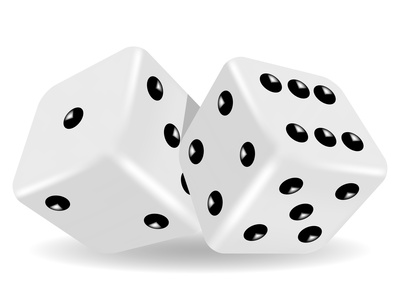
\includegraphics[width=11em]{de.jpg}\\[30cm]
        \end{center}
    \end{Large}
\newpage

\section{Description du jeu}
\paragraph{}
    \begin{large}
        Deux joueurs s'affrontent dans un jeu de dés. Le but est d'être le premier à atteindre au moins
        N points.Le nombre de points marqués est 1 si l'un des dés au moins tombe sur 1,
        dans le cas contraire c'est la somme des dés. On dit qu'un joueur a un gain égal à 1 s'il remporte la partie, un gain égal
        à 0 si la partie est nulle, un gain égal à -1 s'il perd.\\
        Dans ce projet on va étudier deux variante:\\
        - variante séquentielle : les joueurs jouent à tour de rôle;\\
        - variante simultanée : les joueurs jouent simultanément à chaque tour. Dans ce cas si les
        deux joueurs atteignent N points ou plus lors du même tour, c'est le joueur qui dépasse le
        plus les N points qui l'emporte; si les deux joueurs obtiennent le même score, alors ils sont
        ex-aequo.
    \end{large}
\section{Probabilités}
\paragraph{}
    \begin{large}
        Soit P(d,k) la probabilité qu'un joueur qui lance d dés obtienne k points. Donc:\\
        - P(d,1)=1-$(\frac{5}{6})^{d}$: c'est la probabilité qu'au moins un dé tombe sur 1.\\
        - P(d, k) = 0 pour $2 \le k \le 2d$-1 et pour $k \textgreater 6d$.\\
        - P(d, k) =$(\frac{5}{6})^{d}Q(d,k)$ pour $2d \le k \le 6d$ avec Q(d,k) est la probabilité d'obtenir k points en jetant d dés sachant qu'aucun dé n'est tombé sur 1. Q(d,k) peut se calculer à l'aide de la formule de récurrence suivante pour $d \ge 2$ et $2d \le k \le 6d$: $Q(d,k)= \sum_{j=2}^{6} \frac{Q(d-1,k-j)}{5}$.\\
        
        \underline{Explication :} Si l'on obtient k points en lançant le dieme dè alors on a deja obtenue k' dés aprés avoir lancé d-1 dés telque k' ne peut prendre que des valeurs allant de k-2 à k-6, on a donc 5 cas probables avec chaqu'un une probabilité P(d-1,k') donc chaque cas à une probabilité $(\frac{5}{6})$P(d-1,k') . La probabilité d'avoir k point en lancant d dès est donc la somme des probabilité des états qui l'induisent. Donc on a bien $Q(d,k)= \sum_{j=2}^{6} \frac{Q(d-1,k-j)}{5}$.\\
        
        \underline{Cas d'initialisation :} $Q(1,k)=(\frac{1}{5})$ pour k=2,...,6
    \end{large}
    
\section{Variante séquentielle}

\subsection{Stratégie aveugle}
\paragraph{}
    \begin{large}
    La stratégie aveugle consiste à lancer d dès telque d représente le nombre de dès qui maximise l'espérance EP(d)=$4d(\frac{5}{6})^{d}+1-(\frac{5}{6})^{d}$ du nombre de points obtenus.\\
    
    Cette stratégie n'est pas optimale.\\
    Posons N=100, D=10, les deux joueurs étants dans un état (i,j)=(98,94) et c'est le tour du joueur 1 de jouer. D'aprés la stratégie aveugle le joueur devrait lancer 6 dés, sa probabilité de gagner serait donc $\sum_{k=2}^{36}P(6,k)$. D'aprés la table P construite précédement (question 1) cette somme de probabilité est égale à 0.335, or si le joueur lance un seul dé il a une chance $\frac{5}{6}=0,833$ de gagner. On en conclu que cette stratégie n'est pas optimale.
    \end{large}


    \subsection{Programmation dynamique}

    \paragraph{}
      \begin{large}
        Dans cette section, on calcule une stratégie en se basant sur la programmation dynamique. Il s'agit 
        de construire une table EG de dimensions (N-1+6D)x(N-1+6D) resprésentant l'éspérance de gain dans un état (i,j) tel que: 
        état(i,j) : état où le premier joueur a cumulé i points, le deuxième joueur a cumulé j
        points, et c'est au joueur 1 de jouer.
        \paragraph{\large{Formule de récurrence: }} \\
        Le jeu étant à somme nulle, l'espérance de gain du joueur 1 est égale à (-) l'espérance de gain de son adversaire. Étant un état (i,j),
        le joueur 2 calcule son espérance de gain, pour un 'd' donné que lance le joueur 1, de la manière suivante:\\
        EG2(j,i)=$\sum_{k=1}^{6d} {P(d,k)EG1(j,i+k)}$ .\\
        Les deux joeurs jouent de façon optimale, la même table est utilisée, et donc le joueur 1 
        est en mesure de calculer EG2 et de joueur de façon à minimiser cet espérance. On aura donc : \\
        EG1(i,j) = - min (EG2(j,i)) = - min($\sum_{k=1}^{6d} {P(d,k)EG(j,i+k)}$) \\
        \underline{Initialisation:}\\
        Si on est dans un état où $i \ge N$ alors soit il a gagné ( $i \ge j$ ), soit il a perdu ( $i \le j$ ), soit la partie est nulle ( i = j ). \\
                $$
            \ EG(i,j) = \left\{
                \begin{array}{ll}
                    1 & \mbox{si  } i>j, i\ge N \\
                    -1 & \mbox{si } i<j, j\ge N  \\
                    0 & \mbox{si  } i=j, i\ge N 
                \end{array}
            \right.
            $$
        \paragraph{La stratégie optimale: } \\
        Cette approche permet de trouver la stratégie optimale dans chaque état. Il suffit, lors du calcul 
        de l'espérance de gain, de sauvegarder le nombre de dés 'd' permettant d'obtenir ce résultat. 
        \paragraph{Difficulté possible: }
        Si on supposait que le nombre de points marqués est 0 (et non plus 1) si on obtient au moins un 1, 
        les points cumulés par les joueurs risquent à ne pas changer pendant plusieurs tours. C'est à dire,
        l'algorithme reste dans un état (i,j), et ça pour une durée indéterminée, voir à l'infinie. Donc l'algorithme risque à ne pas se terminer.
        
        \subsection{Mise en oeuvre}
        \paragraph{Implémentation: }
        On implémente trois stratégies: \\
        \underline{Stratégie aveugle:}\\
        Il s'agit de retourner le 'd' qui maximise la fonction de l'espérance.\\
        \underline{Stratégie optimale:}\\
        En plus de la table EG, la fonction retourne une table 'strat' de même dimension qui donne 
        le nombre de dés optimal à jouer dans chaque état.\\ 
        \underline{Stratégie aléatoire:}\\
        On implémente de plus une stratégie aléatoire qui retoune aléatoirement un nombre entre 1 et D de dés à jouer. \\
        \paragraph{Evaluation: }\\
        On simule plusieurs parties où le joueur 1 utilise une des trois stratégies contre une autre et on calcule son espérance de gain :\\
        \underline{En variant N: } on fixe D à une valeur passée en argument (ici D=10),et pour 
        chaque valeur de N, on  et on compte le gain du joueur 1.\\ 
        
        \subfloat{{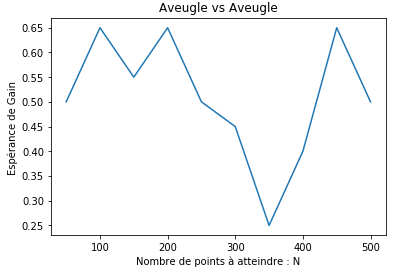
\includegraphics[width=7cm]{Na_a.png} }}
        \qquad
        \subfloat{{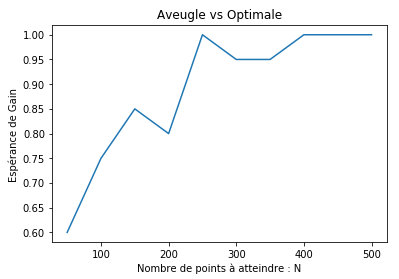
\includegraphics[width=7cm]{Na_o.png} }}
        \\[1em]
        \subfloat{{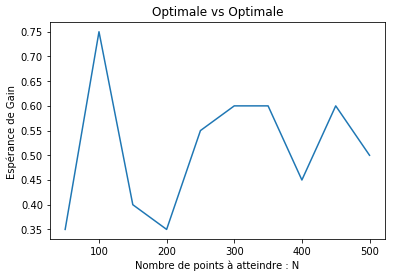
\includegraphics[width=7cm]{No_o.png} }}
        \qquad
        \subfloat{{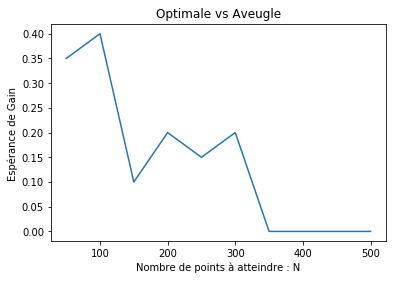
\includegraphics[width=7cm]{No_a.png} }}
        \\[1em]
        \subfloat{{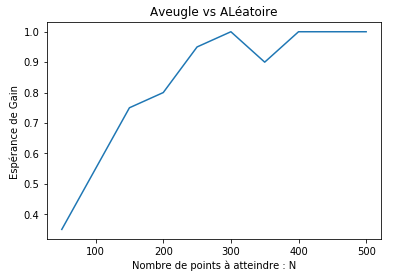
\includegraphics[width=7cm]{Na_r.png} }}
        \qquad
        \subfloat{{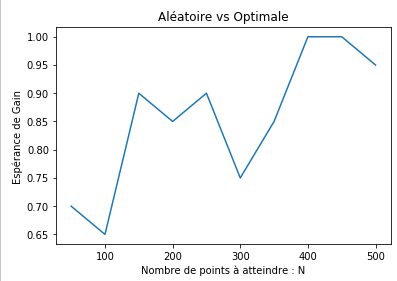
\includegraphics[width=7cm]{Nr_o.png} }} \\[1.5em]
    
        On générale, on constate que la stratégie aveugle donne des bons résultats contre les autres 
        stratégies avec un espérance de gain plus en plus sûr en augmentant N. \\
    
        \underline{En variant D: } on fixe N à une valeur passée en argument (ici N=50),et pour 
        chaque valeur de D, et on compte le gain du joueur 1.\\
      
        \subfloat{{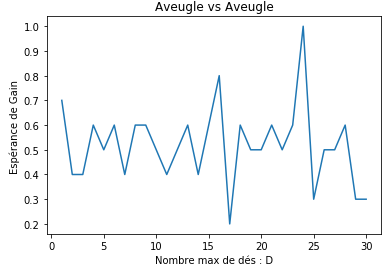
\includegraphics[width=7cm]{Da_a.png} }}
        \qquad
        \subfloat{{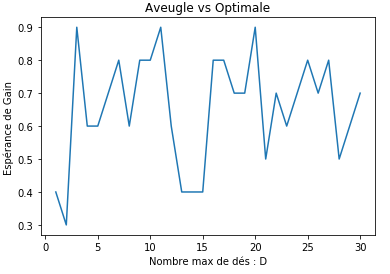
\includegraphics[width=7cm]{Da_o.png} }}
        \\[1em]
        \subfloat{{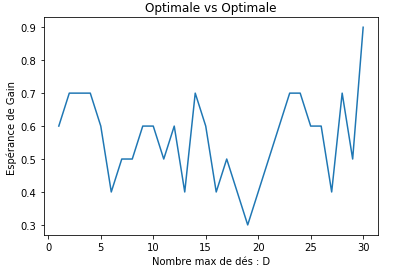
\includegraphics[width=7cm]{Do_o.png} }}
        \qquad
        \subfloat{{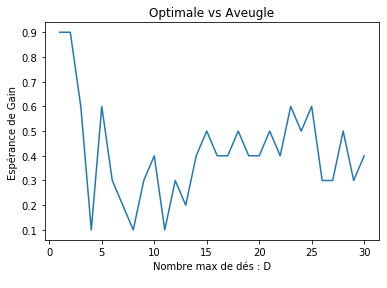
\includegraphics[width=7cm]{Do_a.png} }}
        \\[1em]
        \subfloat{{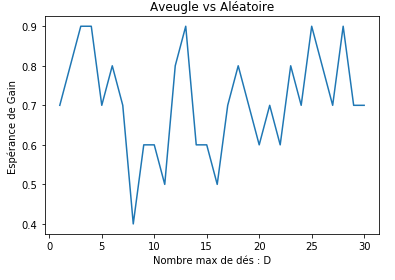
\includegraphics[width=7cm]{Da_r.png} }}
        \qquad
        \subfloat{{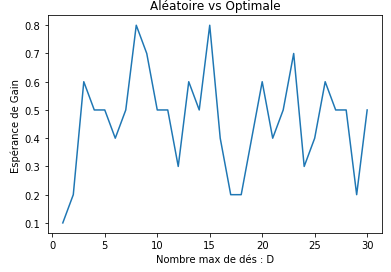
\includegraphics[width=7cm]{Dr_o.png} }}\\[1.5em]
         Pour les différentes stratégies, la variation de D entre une variation non-monotone de l'espérance de gain.
    
         \paragraph{Interface de jeu: }\\
          L'interface ci-desous permet de jouer contre l'ordinateur pour N=100 et D=5.\\[2em]
    
    
         \centering
          \subfloat{{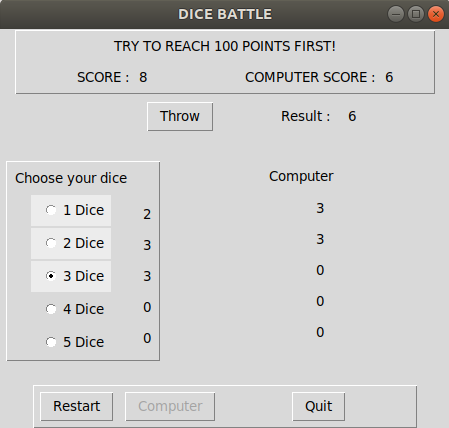
\includegraphics[width=20em]{jeu.png} }}\\
         
      \end{large}
  

\section{Variante simultanée}
    \large{
    Si les deux joueurs jouent à chaque tour de façon simultanée, alors la stratégie optimale dans un état(i,j) donné est randomisée. Ainsi, nous considérons des stratégies randomisées, consistant à donner un vecteur p= [p(1), p(2), . . . , p(D)] où p(d) est la probabilité avec laquelle nous lançons d dés.}
    
\subsection{Jeu en un coup}
    \large{
    On considère en première approche une version simplifiée où l'on ne lance qu'une fois les dés. Le gagnant est simplement celui qui remporte le plus de points.\\
    \paragraph{Espérance de gain} On note EG1(d1,d2) l'espérance de gain du joueur 1 s'il lance d1 dés alors que le joueur 2 en lance d2.\\
    On a donc : EG1(d1,d2)= $\sum_{k1=1}^{6d1} {kP(d1,k1) - \sum_{k2=1}^{6d2} {kP(d2,k2)}$, représentant le nombre de points gagnés (k1) fois la probabilité de gagner k1 points en lançant d1 dés pour le joueur 1 moins la perte (k2) fois la probabilité de perte qui n'est autre que la probabilité de gain du joeur 2 en lançant d2 dès puisque le jeu est à somme nulle.\\
    Pour D=3, on a la matrice de gain suivante :\\
    

        \begin{center}
        \begin{tabular}{ |c|c|c|c| } 
        \hline
        EG1(d1,d2) & 1 & 2 & 3 \\ 
        \hline
        1 & 0 & -2.36111111 & -3.86574074\\ 
        \hline
        2 & 2.36111111 & 0 & -1.50462963\\ 
        \hline
        3 & 3.86574074 & 1.50462963 & 0 \\ 
        \hline
        \end{tabular}
        \end{center}

    \paragraph{Stratégie optimale du joueur 2} Si le joueur 2 connaît la stratégie du joueur 1 : le vecteur de probabilités [p1(1), p1(2), . . . , p1(D)], sa stratégie optimale consisterait donc à minimiser les gains de son adversaire. 
    $\displaystyle \min_{dj} ( \sum_{i=1}^{D} {p1(di)EG1(di,dj)} )$, i,j=1,...,D.\\

    \paragraph{Maximiser l'éspérance de gain du joueur 1} Le joueur 1 cherche à maximiser son gain, sachant que le joeur 2
    répond lui aussi de façon optimale, il chercherait donc à maximiser le sien en minimisant le gain du premier joueur comme vu precédement $\displaystyle \min_{dj} ( \sum_{i=1}^{D} {p1(di)EG1(di,dj)} )$ et donc le joueur 1 aurait intérêt à maximiser : $\displaystyle \max_{di} ( \min_{dj} ( \sum_{i=1}^{D} {p1(di)EG1(di,dj)} ) )$, i,j=1,...,D.\\
    \paragraph{Programme Lineaire}
    
    \begin{equation*}
    \begin{array}{ll@{}ll}
    \text{Max}  & \displaystyle Z &\\
    \text{contraintes}& \displaystyle Z\le\sum_{i=1}^{D} {p1(di)EG1(di,dj)}&, j=1 ,..., D\\&pi\ge0 &, i=1 ,..., D
    \end{array}
    \end{equation*}

    \paragraph{Comparaison entre la stratégie Optimale et la stratégie deterministe Aveugle}
    Pour D=1,...,30\\
    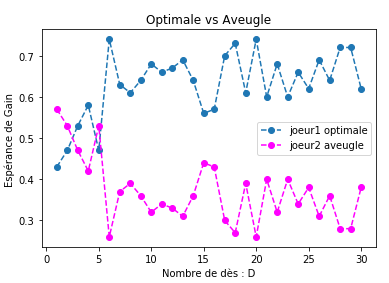
\includegraphics[width=15em]{OA.png} \\
    On voit bien que l'espérance de gain pour la stratégie optimale varie entre 0,75 et 0,6 contre 0,3 à 0,4 pour la stratégie aveugle. 

\subsection{Cas général}
\large{
Dans cette partie on va étendre notre stratégie randomisée au cas général de notre jeu où il s'agit de dépasser N points.
\paragraph{Esperance de gain du joeur 1} L'espérance de gain EG1(i,j) du joueur 1 lorsque $i\ge N$ ou $j\ge N$ est calculé comme suit : $EG1(i,j)=\frac{i-j}{|i-j|}$ si $i\neq j$, 0 sinon. 

\paragraph{Espérance de gain $\displaystyle E^{d1,d2}$(i,j) du joueur 1}
Soit EG1(k,l) l'espérance de gain du joueur 1  lorsque $k\textgreater i$ et $l\textgreater j$ (lorsque les joueurs jouent de manière optimale).\\
Supposons que le joueur 1 lance d1 dés et que le joueur 2 lance d2 dés. L'espérance de gain du joeur 1 est donnée comme suit : \\
$\displaystyle E^{d1,d2}$(i,j)=$\sum_{k1=1}^{6d1} \sum_{k2=1}^{6d2}{P(d1,k1)P(d2,k2)EG(i+k1,j+k2)}$.
\paragraph{Espérance de gain EG(i,j) du joueur 1}
Par la suite le calcule de EG se fait en appliquant la résolution linéaire à $\displaystyle E^{d1,d2}$, pour chaque
case EG(i,j). \\
La stratégie optimale retournée pour l'état (i,j) étant le vecteur p retourné par la résolution linéaire.
}

}

\section{Conclusion}
On a pu étudier tout au long du projet trois stratégies pour le jeu Dice Battle. En sequentiel on a vu une premiere strategie Aveugle qui n'est pas optimale néaumoins facile à implémenter, la stratégie dynamique quant à elle fournit de meilleurs résultats mais nécéssite le cacul des probabilités de gains à partir de chaque état possible. En simultané, notre stratégie randomisée fournie de bons résultats contre une stratégie aléatoire ou aveugle, mais pour un adversaire utilisant la même approche on obtient un gain nul puisque le jeu est à somme nulle. 

\end{document}


